\begin{figure}[t]
\centering
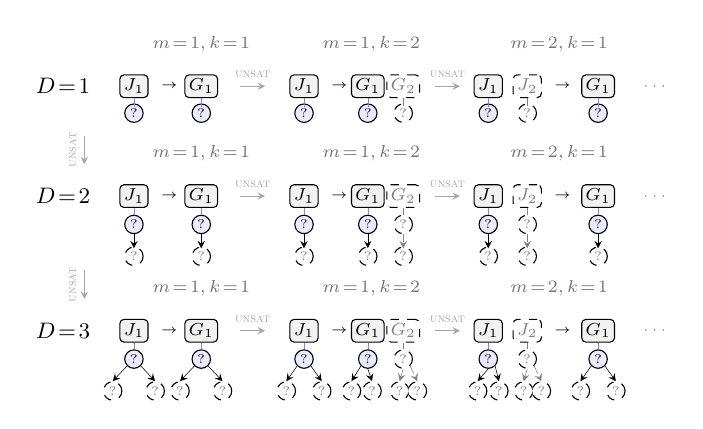
\begin{tikzpicture}[scale=0.9, every node/.style={transform shape},
  skel/.style={font=\scriptsize, draw, rounded corners=1.5pt,
               minimum height=0.32cm, inner sep=1.5pt, fill=gray!10},
  skeldash/.style={font=\scriptsize, draw, dashed, rounded corners=1.5pt,
               minimum height=0.32cm, inner sep=1.5pt, fill=white, text=gray},
  temporal/.style={font=\scriptsize},
  dagnode/.style={draw, circle, minimum size=0.26cm, inner sep=0pt,
                  font=\tiny, fill=blue!8},
  dagdash/.style={draw, circle, minimum size=0.26cm, inner sep=0pt,
                  font=\tiny, dashed, fill=white, text=gray},
   dagdot/.style={draw, circle, minimum size=0.26cm, inner sep=0pt,
                  font=\tiny, dotted, fill=white, text=gray},
  conn/.style={-, very thin, blue!50},
  arr/.style={->, >=stealth, very thin},
  darr/.style={->, >=stealth, very thin, dashed, gray},
  lbl/.style={draw=none, font=\small\bfseries},
  note/.style={draw=none, font=\tiny, text=black!55},
  uarr/.style={->, >=stealth, very thin, black!35},
]
% spacing constants
\def\colA{0.6}
\def\colB{3.0}
\def\colC{5.7}
\def\dotsX{7.5}
% vertical spacing
\def\rA{0}       % D=1 skeleton y
\def\rB{-1.55}   % D=2 skeleton y
\def\rC{-3.45}   % D=3 skeleton y
% D=2 chain spacing
\def\chH{0.45}   % chain node gap

% ========== D=1 ROW ==========
\node[lbl] at (-0.85, \rA) {$D\!=\!1$};

% --- m=1,k=1 ---
\node[note] at (\colA+0.5, \rA+0.6) {\scriptsize$m\!=\!1,k\!=\!1$};
\node[temporal] at (\colA-0.45, \rA+0.28) {\tiny$\always\eventually$};
\node[skel] (j1a) at (\colA-0.45, \rA) {$J_1$};
\node[temporal] at (\colA+0.05, \rA) {\tiny$\to$};
\node[temporal] at (\colA+0.5, \rA+0.28) {\tiny$\always\eventually$};
\node[skel] (g1a) at (\colA+0.5, \rA) {$G_1$};
\node[dagnode] at (\colA-0.45, \rA-0.38) {$?$};
\node[dagnode] at (\colA+0.5, \rA-0.38) {$?$};
\draw[conn] (j1a.south) -- ++(0,-0.13);
\draw[conn] (g1a.south) -- ++(0,-0.13);

\draw[uarr] (\colA+1.05, \rA) -- node[above, font=\tiny, text=black!35]
  {\textsc{unsat}} ++(0.35, 0);

% --- m=1,k=2 ---
\node[note] at (\colB+0.5, \rA+0.6) {\scriptsize$m\!=\!1,k\!=\!2$};
\node[temporal] at (\colB-0.45, \rA+0.28) {\tiny$\always\eventually$};
\node[skel] (j1b) at (\colB-0.45, \rA) {$J_1$};
\node[temporal] at (\colB+0.05, \rA) {\tiny$\to$};
\node[temporal] at (\colB+0.45, \rA+0.28) {\tiny$\always\eventually$};
\node[skel] (g1b) at (\colB+0.45, \rA) {$G_1$};
\node[temporal] at (\colB+0.95, \rA+0.28) {\tiny$\always\eventually$};
\node[skeldash] (g2b) at (\colB+0.95, \rA) {$G_2$};
\node[dagnode] at (\colB-0.45, \rA-0.38) {$?$};
\node[dagnode] at (\colB+0.45, \rA-0.38) {$?$};
\node[dagdash] at (\colB+0.95, \rA-0.38) {$?$};
\draw[conn] (j1b.south) -- ++(0,-0.13);
\draw[conn] (g1b.south) -- ++(0,-0.13);
\draw[conn, dashed, gray] (g2b.south) -- ++(0,-0.13);

\draw[uarr] (\colB+1.4, \rA) -- node[above, font=\tiny, text=black!35]
  {\textsc{unsat}} ++(0.35, 0);

% --- m=2,k=1 ---
\node[note] at (\colC+0.45, \rA+0.6) {\scriptsize$m\!=\!2,k\!=\!1$};
\node[temporal] at (\colC-0.55, \rA+0.28) {\tiny$\always\eventually$};
\node[skel] (j1c) at (\colC-0.55, \rA) {$J_1$};
\node[temporal] at (\colC+0.0, \rA+0.28) {\tiny$\always\eventually$};
\node[skeldash] (j2c) at (\colC+0.0, \rA) {$J_2$};
\node[temporal] at (\colC+0.5, \rA) {\tiny$\to$};
\node[temporal] at (\colC+1.0, \rA+0.28) {\tiny$\always\eventually$};
\node[skel] (g1c) at (\colC+1.0, \rA) {$G_1$};
\node[dagnode] at (\colC-0.55, \rA-0.38) {$?$};
\node[dagdash] at (\colC+0.0, \rA-0.38) {$?$};
\node[dagnode] at (\colC+1.0, \rA-0.38) {$?$};
\draw[conn] (j1c.south) -- ++(0,-0.13);
\draw[conn, dashed, gray] (j2c.south) -- ++(0,-0.13);
\draw[conn] (g1c.south) -- ++(0,-0.13);

\node[note] at (\dotsX, \rA) {$\cdots$};

% ========== down arrow ==========
\draw[arr, black!35] (-0.55, \rA-0.7) --
  node[left, font=\tiny, text=black!35] {\rotatebox{90}{\textsc{unsat}}}
  (-0.55, \rB+0.45);

% ========== D=2 ROW ==========
\node[lbl] at (-0.85, \rB) {$D\!=\!2$};

% --- m=1,k=1 ---
\node[note] at (\colA+0.5, \rB+0.6) {\scriptsize$m\!=\!1,k\!=\!1$};
\node[temporal] at (\colA-0.45, \rB+0.28) {\tiny$\always\eventually$};
\node[skel] (j1d) at (\colA-0.45, \rB) {$J_1$};
\node[temporal] at (\colA+0.05, \rB) {\tiny$\to$};
\node[temporal] at (\colA+0.5, \rB+0.28) {\tiny$\always\eventually$};
\node[skel] (g1d) at (\colA+0.5, \rB) {$G_1$};
\node[dagnode] (d2j1r) at (\colA-0.45, \rB-0.4) {$?$};
\node[dagdash] at (\colA-0.45, \rB-0.4-\chH) {$?$};
\draw[arr] (d2j1r.south) -- ++(0,-0.2);
\draw[conn] (j1d.south) -- (d2j1r.north);
\node[dagnode] (d2g1r) at (\colA+0.5, \rB-0.4) {$?$};
\node[dagdash] at (\colA+0.5, \rB-0.4-\chH) {$?$};
\draw[arr] (d2g1r.south) -- ++(0,-0.2);
\draw[conn] (g1d.south) -- (d2g1r.north);

\draw[uarr] (\colA+1.05, \rB) -- node[above, font=\tiny, text=black!35]
  {\textsc{unsat}} ++(0.35, 0);

% --- m=1,k=2 ---
\node[note] at (\colB+0.5, \rB+0.6) {\scriptsize$m\!=\!1,k\!=\!2$};
\node[temporal] at (\colB-0.45, \rB+0.28) {\tiny$\always\eventually$};
\node[skel] (j1e) at (\colB-0.45, \rB) {$J_1$};
\node[temporal] at (\colB+0.05, \rB) {\tiny$\to$};
\node[temporal] at (\colB+0.45, \rB+0.28) {\tiny$\always\eventually$};
\node[skel] (g1e) at (\colB+0.45, \rB) {$G_1$};
\node[temporal] at (\colB+0.95, \rB+0.28) {\tiny$\always\eventually$};
\node[skeldash] (g2e) at (\colB+0.95, \rB) {$G_2$};
\node[dagnode] (d2j1er) at (\colB-0.45, \rB-0.4) {$?$};
\node[dagdash] at (\colB-0.45, \rB-0.4-\chH) {$?$};
\draw[arr] (d2j1er.south) -- ++(0,-0.2);
\draw[conn] (j1e.south) -- (d2j1er.north);
\node[dagnode] (d2g1er) at (\colB+0.45, \rB-0.4) {$?$};
\node[dagdash] at (\colB+0.45, \rB-0.4-\chH) {$?$};
\draw[arr] (d2g1er.south) -- ++(0,-0.2);
\draw[conn] (g1e.south) -- (d2g1er.north);
\node[dagdash] (d2g2er) at (\colB+0.95, \rB-0.4) {$?$};
\node[dagdash] at (\colB+0.95, \rB-0.4-\chH) {$?$};
\draw[darr] (d2g2er.south) -- ++(0,-0.2);
\draw[conn, dashed, gray] (g2e.south) -- (d2g2er.north);

\draw[uarr] (\colB+1.4, \rB) -- node[above, font=\tiny, text=black!35]
  {\textsc{unsat}} ++(0.35, 0);

% --- m=2,k=1 ---
\node[note] at (\colC+0.45, \rB+0.6) {\scriptsize$m\!=\!2,k\!=\!1$};
\node[temporal] at (\colC-0.55, \rB+0.28) {\tiny$\always\eventually$};
\node[skel] (j1f2) at (\colC-0.55, \rB) {$J_1$};
\node[temporal] at (\colC+0.0, \rB+0.28) {\tiny$\always\eventually$};
\node[skeldash] (j2f2) at (\colC+0.0, \rB) {$J_2$};
\node[temporal] at (\colC+0.5, \rB) {\tiny$\to$};
\node[temporal] at (\colC+1.0, \rB+0.28) {\tiny$\always\eventually$};
\node[skel] (g1f2) at (\colC+1.0, \rB) {$G_1$};
\node[dagnode] (d2j1fr) at (\colC-0.55, \rB-0.4) {$?$};
\node[dagdash] at (\colC-0.55, \rB-0.4-\chH) {$?$};
\draw[arr] (d2j1fr.south) -- ++(0,-0.2);
\draw[conn] (j1f2.south) -- (d2j1fr.north);
\node[dagdash] (d2j2fr) at (\colC+0.0, \rB-0.4) {$?$};
\node[dagdash] at (\colC+0.0, \rB-0.4-\chH) {$?$};
\draw[darr] (d2j2fr.south) -- ++(0,-0.2);
\draw[conn, dashed, gray] (j2f2.south) -- (d2j2fr.north);
\node[dagnode] (d2g1fr) at (\colC+1.0, \rB-0.4) {$?$};
\node[dagdash] at (\colC+1.0, \rB-0.4-\chH) {$?$};
\draw[arr] (d2g1fr.south) -- ++(0,-0.2);
\draw[conn] (g1f2.south) -- (d2g1fr.north);

\node[note] at (\dotsX, \rB) {$\cdots$};

% ========== down arrow ==========
\draw[arr, black!35] (-0.55, \rB-0.4-\chH-0.2) --
  node[left, font=\tiny, text=black!35] {\rotatebox{90}{\textsc{unsat}}}
  (-0.55, \rC+0.45);

% ========== D=3 ROW ==========
\node[lbl] at (-0.85, \rC) {$D\!=\!3$};
\def\treeS{0.3}  % tree spread

% --- m=1,k=1 ---
\node[note] at (\colA+0.5, \rC+0.6) {\scriptsize$m\!=\!1,k\!=\!1$};
\node[temporal] at (\colA-0.45, \rC+0.28) {\tiny$\always\eventually$};
\node[skel] (j1f) at (\colA-0.45, \rC) {$J_1$};
\node[temporal] at (\colA+0.05, \rC) {\tiny$\to$};
\node[temporal] at (\colA+0.5, \rC+0.28) {\tiny$\always\eventually$};
\node[skel] (g1f) at (\colA+0.5, \rC) {$G_1$};
% J1 tree (solid/blue)
\node[dagnode] (t1jr) at (\colA-0.45, \rC-0.4) {$?$};
\node[dagdash] (t1jl) at (\colA-0.45-\treeS, \rC-0.85) {$?$};
\node[dagdash] (t1jrr) at (\colA-0.45+\treeS, \rC-0.85) {$?$};
\draw[arr] (t1jr.south west) -- (t1jl.north);
\draw[arr] (t1jr.south east) -- (t1jrr.north);
\draw[conn] (j1f.south) -- (t1jr.north);
% G1 tree (solid/blue)
\node[dagnode] (t1gr) at (\colA+0.5, \rC-0.4) {$?$};
\node[dagdash] (t1gl) at (\colA+0.5-\treeS, \rC-0.85) {$?$};
\node[dagdash] (t1grr) at (\colA+0.5+\treeS, \rC-0.85) {$?$};
\draw[arr] (t1gr.south west) -- (t1gl.north);
\draw[arr] (t1gr.south east) -- (t1grr.north);
\draw[conn] (g1f.south) -- (t1gr.north);

\draw[uarr] (\colA+1.05, \rC) -- node[above, font=\tiny, text=black!35]
  {\textsc{unsat}} ++(0.35, 0);

% --- m=1,k=2 ---
\node[note] at (\colB+0.5, \rC+0.6) {\scriptsize$m\!=\!1,k\!=\!2$};
\node[temporal] at (\colB-0.45, \rC+0.28) {\tiny$\always\eventually$};
\node[skel] (j1g) at (\colB-0.45, \rC) {$J_1$};
\node[temporal] at (\colB+0.05, \rC) {\tiny$\to$};
\node[temporal] at (\colB+0.45, \rC+0.28) {\tiny$\always\eventually$};
\node[skel] (g1g) at (\colB+0.45, \rC) {$G_1$};
\node[temporal] at (\colB+0.95, \rC+0.28) {\tiny$\always\eventually$};
\node[skeldash] (g2g) at (\colB+0.95, \rC) {$G_2$};
% J1: left+right (solid, like m=1,k=1)
\node[dagnode] (t2jr) at (\colB-0.45, \rC-0.4) {$?$};
\node[dagdash] (t2jl) at (\colB-0.7, \rC-0.85) {$?$};
\node[dagdash] (t2jrr) at (\colB-0.2, \rC-0.85) {$?$};
\draw[arr] (t2jr.south west) -- (t2jl.north);
\draw[arr] (t2jr.south east) -- (t2jrr.north);
\draw[conn] (j1g.south) -- (t2jr.north);
% G1: left+center (solid)
\node[dagnode] (t2g1r) at (\colB+0.45, \rC-0.4) {$?$};
\node[dagdash] (t2g1l) at (\colB+0.22, \rC-0.85) {$?$};
\node[dagdash] (t2g1c) at (\colB+0.51, \rC-0.85) {$?$};
\draw[arr] (t2g1r.south west) -- (t2g1l.north);
\draw[arr] (t2g1r.south) -- (t2g1c.north);
\draw[conn] (g1g.south) -- (t2g1r.north);
% G2: center+right (dashed)
\node[dagdash] (t2g2r) at (\colB+0.95, \rC-0.4) {$?$};
\node[dagdash] (t2g2c) at (\colB+0.9, \rC-0.85) {$?$};
\node[dagdash] (t2g2rr) at (\colB+1.15, \rC-0.85) {$?$};
\draw[darr] (t2g2r.south) -- (t2g2c.north);
\draw[darr] (t2g2r.south east) -- (t2g2rr.north);
\draw[conn, dashed, gray] (g2g.south) -- (t2g2r.north);

\draw[uarr] (\colB+1.4, \rC) -- node[above, font=\tiny, text=black!35]
  {\textsc{unsat}} ++(0.35, 0);

% --- m=2,k=1 ---
\node[note] at (\colC+0.45, \rC+0.6) {\scriptsize$m\!=\!2,k\!=\!1$};
\node[temporal] at (\colC-0.55, \rC+0.28) {\tiny$\always\eventually$};
\node[skel] (j1h) at (\colC-0.55, \rC) {$J_1$};
\node[temporal] at (\colC+0.0, \rC+0.28) {\tiny$\always\eventually$};
\node[skeldash] (j2h) at (\colC+0.0, \rC) {$J_2$};
\node[temporal] at (\colC+0.5, \rC) {\tiny$\to$};
\node[temporal] at (\colC+1.0, \rC+0.28) {\tiny$\always\eventually$};
\node[skel] (g1h) at (\colC+1.0, \rC) {$G_1$};
% J1: center+right children (solid)
\node[dagnode] (t3j1r) at (\colC-0.55, \rC-0.4) {$?$};
\node[dagdash] (t3j1c) at (\colC-0.7, \rC-0.85) {$?$};
\node[dagdash] (t3j1rr) at (\colC-0.4, \rC-0.85) {$?$};
\draw[arr] (t3j1r.south) -- (t3j1c.north);
\draw[arr] (t3j1r.south east) -- (t3j1rr.north);
\draw[conn] (j1h.south) -- (t3j1r.north);
% J2: center+right children (dashed)
\node[dagdash] (t3j2r) at (\colC+0.0, \rC-0.4) {$?$};
\node[dagdash] (t3j2c) at (\colC-0.05, \rC-0.85) {$?$};
\node[dagdash] (t3j2rr) at (\colC+0.2, \rC-0.85) {$?$};
\draw[darr] (t3j2r.south) -- (t3j2c.north);
\draw[darr] (t3j2r.south east) -- (t3j2rr.north);
\draw[conn, dashed, gray] (j2h.south) -- (t3j2r.north);
% G1: left+right children (solid)
\node[dagnode] (t3g1r) at (\colC+1.0, \rC-0.4) {$?$};
\node[dagdash] (t3g1l) at (\colC+0.75, \rC-0.85) {$?$};
\node[dagdash] (t3g1rr) at (\colC+1.25, \rC-0.85) {$?$};
\draw[arr] (t3g1r.south west) -- (t3g1l.north);
\draw[arr] (t3g1r.south east) -- (t3g1rr.north);
\draw[conn] (g1h.south) -- (t3g1r.north);

\node[note] at (\dotsX, \rC) {$\cdots$};

\end{tikzpicture}
\caption{Two-dimensional search in \toolname.
\textbf{Horizontal}: template enumeration over $(m,k)$ via
push/pop.
\textbf{Vertical}: propositional depth $D$.
$D\!=\!1$: single leaves.
$D\!=\!2$: chains (one operator).
$D\!=\!3$: trees ($\lnot x_0 \land x_1$, etc.).
Solid = current; dashed = newly added.}\label{fig:search}
\end{figure}

